\begin{center}{ \bf ИНТЕГРИРУЕМЫЕ БИЛЛИАРДНЫЕ КНИЖКИ МОДЕЛИРУЮТ 3-АТОМЫ И ГРУБЫЕ МОЛЕКУЛЫ}\\
{\it И.\,С. Харчева } \\
(Москва; {\it irina\_harcheva@mail.ru})
\end{center}
\addcontentsline{toc}{section}{Иванов И.И.}


Опишем стандартную постановку биллиардной задачи в некоторой области на плоскости. Пусть дана связная плоская компактная область $\Omega$, ограниченная замкнутой кусочно-гладкой кривой. При этом все углы в точках излома границы равны $\pi/2$ и кривая не предполагается связной.
Пусть материальная точка (биллиардный шар) движется внутри области $\Omega$ и отражается на границе по естественному закону
(угол падения равен углу отражения) При этом в точках излома границы движение очевидно продолжается по непрерывности, так как угол излома равен $ \pi/2 $.
Как известно, эта динамика задает гамильтонову систему на кокасательном расслоении к области $\Omega$.  При этом точка этого расслоения задаётся координатами материальной точки в области и кокасательным (касательным, поскольку метрика плоская) вектором в данной точке.
Эта система обладает естественным интегралом -- модулем вектора скорости. В некоторых случаях она имеет также
второй независимый интеграл. Примером является биллиард в области $\Omega$, ограниченной дугами софокусных эллипсов и гипербол. Оказывается, в таком биллиарде вектор скорости материальной точки на протяжении всей траектории будет направлен по касательной к фиксированной квадрике, софокусной с семейством. Поэтому у такой системы появляется еще один интеграл, независимый с предыдущим -- параметр квадрики $ \Lambda $. Это означает, что динамическая система биллиарда в такой области будет интегрируема по Лиувиллю. Ее интегрируемость была показана в работе В.\,В.~Козловa, Д.\,В.~Трещёвa [1].

Расширим постановку биллиардной задачи. Пусть дано n областей $\Omega_1, ... ,\Omega_n$ с кусочно-гладкой границей.
Пусть граница этих областей содержит одну и ту же кривую $l$ как часть границы. Припишем к этой дуге перестановку $ \sigma $ из n элементов. Тогда можно определить более сложный биллиард в объединении областей $\cup_{i = 1}^n \Omega_i$ следующим образом: материальная точка отражается обычным образом от границ, отличных от $l$ и переходит с одной области на другую по перестановке $ \sigma $, достигая кривой $l$. Заметим, что общих граничных кривых у областей может быть несколько: $ l_1, l_2, ..., l_k $. Ко всем им можно приписать перестановки $ \sigma_1, \sigma_2, ..., \sigma_k $  и рассмотреть биллиард, в котором материальная точка будет переходить с листа на лист на дугах $ l_1, l_2, ..., l_k $ по перестановкам $ \sigma_1, \sigma_2, ..., \sigma_k $ соответственно. Такие биллиарды будем называть \textit{биллиардными книжками}, а области $ \Omega_i $,  из которых состоит биллиардная книжка -- \textit{листами}. В частном случае, когда $ n = 2 $ такие биллиарды называются топологическими. Топологические биллиарды были полностью классифицированы в работе В.В.\,Фокичевой [2]. Классификации в общем случае на нынешний момент нет.

\begin{figure}[h!]
	\center{ 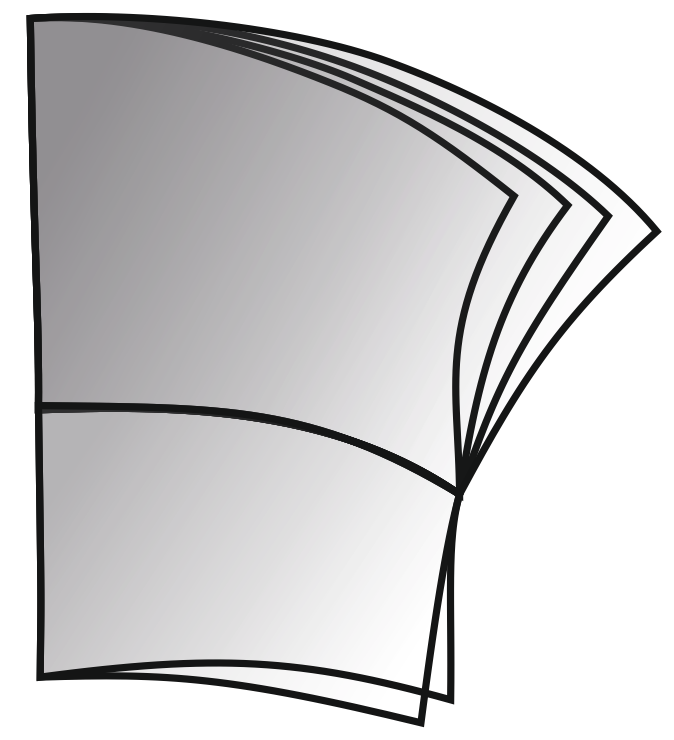
\includegraphics[width=20.5mm]{pic/Khartseva_billbook.png}}
	\caption{Пример биллиардной книжки. \label{3obl}}
\end{figure}

В классификации В.В.\,Фокичевой [2]  было обнаружено, что многие известные и важные интегрируемые системы с двумя степенями свободы моделируются топологическими  биллиардами, то есть их инварианты Фоменко-Цишанга (см. [3]) совпадают. В связи с этим А.Т.\,Фоменко предложил следующую гипотезу:

\textbf{Гипотеза. (А.Т. Фоменко)}
{\it Биллиардными книжками можно моделировать:

	Гипотеза A. все 3-атомы;

	Гипотеза B. все грубые молекулы (инварианты Фоменко);

	Гипотеза C. все меченые молекулы (инварианты Фоменко-Цишанга) .
}

\textbf{Teорема 1. (Ведюшкина-Харчева)}  {\it Гипотеза Фоменко A верна, а именно, для любого 3-атома (со звездочками или без) алгоритмически строится биллиардная книжка, такая что в её изоэнергетической поверхности $ Q^3 $ слоение Лиувилля прообраза окрестности особого значения интеграла $ \Lambda $, отвечающего траекториям, направленным к или от одного из фокусов, послойно гомеоморфно данному атому.}

\textbf{Teорема 2. (Ведюшкина-Харчева)}  {\it Гипотеза Фоменко B верна, а именно, для любой грубой молекулы алгоритмически строится биллиардная книжка, такая что в её изоэнергетической поверхности $ Q^3 $ слоение Лиувилля послойно гомеоморфно данной грубой молекуле.}

\vspace{\baselineskip}
Исследование выполнено за счет гранта Российского научного фонда (проект №17-11-01303).

%%%%  ОФОРМЛЕНИЕ СПИСКА ЛИТЕРАТУРЫ %%%
\smallskip \centerline{\bf Литература}\nopagebreak

1. {\it  Козлов В. В., Трещёв Д.В.} Генетическое введение в динамику систем с ударами. М.:  Изд-во МГУ, 1991. 408 с.

2. {\it Фокичева В. В.} Топологическая классификация биллиардов в локально-плоских областях, ограниченных дугами софокусных квадрик. Математический сборник. — 2015. — Т. 206, № 10. С. 127–176.

3. {\it Болсинов А.В., Фоменко А.Т.} Интегрируемые гамильтоновы системы. Геометрия, топология, классификация, том 1. Ижевск НИЦ "Регулярная и хаотическая динамика", 1999.
